\subsection{\label{sec:sentiment}Sentiment Analysis}
\textbf{Student Name: }Youcef Mammar \textbf{Student ID:} 0873972\\

\subsubsection*{Motivation}
Sentiment analysis is becoming a popular area of research and social media analysis,
especially around user reviews or user interactions involving an opinion about a product
or a company. Identifying opinion polarity, while often not very accurate, is still very
useful and are particularly interesting for companies which want to receive direct (and free)
feedback from their clients.

\subsubsection*{Problem formulation}
Our crawler has gathered a big set of posts, some of them are explicitely related to a brand.
(like contain the username +Microsoft) or product names (like “Surface”). How can we
In the following we will explore some of the options we have to classify a set of posts.



\subsubsection*{Approach}

While there are many possible ways to approach the problem, they all involve some machine learning technique.

Our first try was to use a sentiment dictionary, which for a given words, for a given meaning (part of speech \&
context), could return a polarity score. However the results weren’t as good as expected. The main reason is we
could not easily determine the part of speech of a word or its context, and as we know, the polarity of a word can widely vary depending of theses.

For example, in theses two posts, the word “angry” carries two different meanings which a human can tell only by the context.
\begin{itemize}
 \item ``2 angry customers broke into an apple store last monday'': objective
 \item ``This swiping keyboard really makes me angry'': negative

\end{itemize}


The biggest problem in not being able to identify parts of speech is more visible when we deal with amplifiers
such as “really”. Not knowing which adjective this “really” is attached to makes it difficult to compute a global score for “... really makes me angry”.

Moreover, SentiWordNet didn’t include smileys as words, which could have been very interesting since smileys
express often unambiguously the emotions involved in a tweet.

We won’t go again through explaining how Naive Bayes works since there is a section dedicated to it. But we have
to say that we choose for the sake of simplicity to use a Bernoulli model, which we thought would not have a big
impact since we are dealing with reasonably short texts, where every relevant word (ie not a stop word) will usually appear only once.

The latter method surprisingly gave much better results, after training the classifier on 119783 labeled
sentences (some of them containing smileys). This set of data was obtained by mixing the manually crafted data sets:
“Stanford Sentiment Treebank” and a “twitter sentiment corpus” found on sananalytics.com.

Because our labeled data sets featured only positive and negative posts (no objective posts or any shades of theses),
we had to simplify and focus on 2 only possible classifications: positive and negative.

Input data (training and test data) is cleaned to get rid of irrelevant parts of the content such as punctuation,
misspelled words, urls, \#hashtags, @usernames (twitter) or +usernames (Google+). Also we removed stop words, as the
number of features tend to be very high with Bernoulli method, and working only with the most discriminative is likely
to improve the classification.

We also rely on the spellchecker to correct words such as “Awsuuuuuume”. Smiley and other common words of the internet
such as (“lol”, “haha”, ”arrgh”, etc) are detected and replaced with either the words “smily” or “angry” depending of their
meaning, then processed as regular words. All of this happens during the preprocessing phase.

Then we used Classify.NaiveBayes for the NLTK python package. As a technical detail, the processing of the trained data
(ie the classifier as a python object) is stored on the hard-drive once and for all to speed up the sentiment classification.

\subsubsection*{Evaluation}
We thought that the best way to evaluate our classifier is to try it on part of our labeled data.
We trained the classifier on 80\% of our labeled data set and tested it on the other 20\%.

If for example we want to query for positive posts, we reach then an accuracy of 75\%.


It is safe to say that the best sentiment analysis is done by humans\cite{sentiment_analysis}. However, according to a recent
study conducted at the University of Pittsburgh on Recognizing Contextual Polarity in Phrase-Level Sentiment Analysis\cite{polarity},
humans agree on sentiment only 80\% of the time.

\begin{figure}[h]
\centering
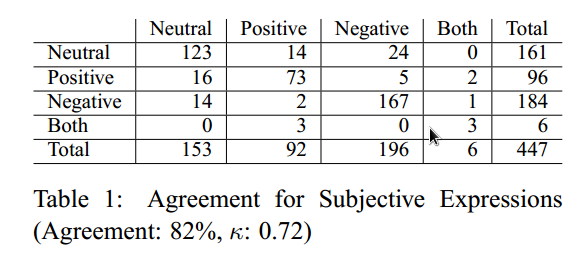
\includegraphics[scale=.5]{images/sent1.png}
\caption{This table is from the \textit{``Recognizing Contextual Polarity in Phrase-Level Sentiment Analysis''}}
\end{figure}

If we look now at the precision and the recall, we find

\begin{description}
 \item[For a positive query]

  precision: 0.908 and
  recall: 0.819


 \item[For a negative query]

  precision: 0.806 and
  recall: 0.899

\end{description}


We can see how precision for negative queries is lower than positive’s. We can explain it by looking at some of the negative posts. 
Negativity are often expressed using the word \textit{“not”} or \textit{``could''} but by basing our classifier only on words, we often miss this forms of negation. 
For this reason, a sentence like \textit{“I’m really not happy with the new iPhone, it could be improved”} could be evaluated to positive and be 
ignored by the query. When a classifier doesn’t catch as much relevant content as it should, we say it has a low recall.

The same way, a sentence like \textit{“Trying out the nexus 5: not bad!”} and other euphemisms which are very common in social talking, would be 
evaluated to negative while it’s positive, leading to a low precision.

\begin{figure}[h]
\centering
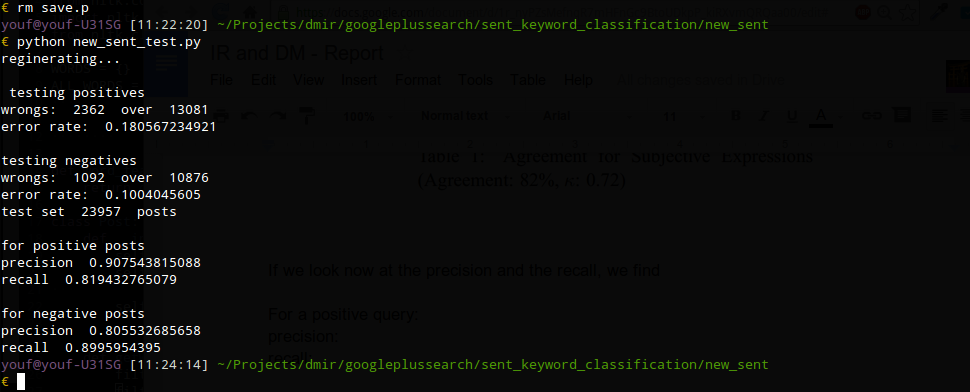
\includegraphics[scale=.4]{images/sent2.png}
\caption{This is the output of the test carried on 23 957 short text samples. It shows the error rate and a other performance figures}
\end{figure}



\subsubsection*{Some outlooks}
\begin{itemize}
 \item
 We could try to work around the bad recall for negative posts using a combination 2-grams and 1-grams as features. This would also help with adverbs that serve as adjective amplifiers.
\item
An even more robust approach could try to use grammar rules to extract the dependecies between the words, though it is arguable that such an approach would work on social media content, as the users tend to use poor grammar.
\item
he words case can contain important information about the emotion of a post as people tend to use caps to evoke anger or sometimes surprise. It certainly would have been an interesting feature if we had more than 2 classes (eg. very negative, negative, objective, positive, very positive). Unfortunately, our data set was limited in that regard.
\item
Bayesien classifiers are relatively very easy to implement and usually give good result with text but it would be interesting to see what we can have with other classifications methods, particularly SVM.

\end{itemize}

